%!TEX root = data-validation-ml-systems.tex
\section{Introduction}
\label{sec:intro}

Machine Learning (ML) technology has become a standard component in modern software systems. Many decisions are increasingly being automated with ML and the predictions of ML models are being exposed in data products or consumed by other downstream software components. This trend gives rise to new research challenges at the intersection between Data Base Management Systems (DBMS) community and the ML community. 
%
Many of these challenges are related to data validation. In contrast to standard software systems, for which a large arsenal of testing concepts and utilities exists, testing of ML systems is difficult. Depending on the ingested data, ML systems can behave very different, and often subtle changes in the input data, that are hard to detect by humans, can lead to very different ML predictions \cite{Athalye18}. 

\newpage
This data dependency in the transformations induced by ML models is their very strength: It allows these systems to adapt to any problem setting by learning from rules defined implicitly by a data set. But this flexibility comes at a cost: The more complex and powerful ML systems become, the more difficult it becomes to validate their predictions. 

For decades ML scientists have been considering data validation rather an engineering challenge than a research problem. Recently however with more ML systems being deployed in customer facing applications newspaper headlines remind us that without proper validation of ML components we will see more racist chatbots\footnote{\scriptsize\url{https://blogs.microsoft.com/blog/2016/03/25/learning-tays-introduction/}} or fatal car crashes\footnote{\scriptsize\url{https://www.nytimes.com/2016/09/15/business/fatal-tesla-crash-in-china-involved-autopilot-government-tv-says.html}}. Scientists in the field are beginning to take this problem very seriously. There is an emergent field of research around data management tailored to ML workflows \cite{Kumar2017}. Testing, monitoring and validation of ML systems and the data ingested and produced by ML models has become a major focus of research with dedicated workshops at major conferences and a rapidly growing research community, as summarized in \autoref{sec:solutions}. Also the recent trend in ML to render models and their predictions more transparent \cite{Samek2019} can be regarded as an attempt to validate ML systems and training or prediction data \cite{Zhang2020}.
%
However to the best of our knowledge there is no commonly agreed upon data validation solution for ML systems that has reached broad adoption. Here, we argue that one of the most important factors is that {\em automating} validation of ML systems is difficult. Especially when systems learn autonomously and continuously, it can be challenging to ensure that the performance of an ML system is not shifting due to accidental or adversarial changes in the data. Given the above examples for how ML systems can fail in practice, it is obvious that ML systems require scalable, robust and automated data validation solutions. This constraint does not apply to academic research, and thus the lack of automation in ML system validation can be considered as a major blocker slowing down the transfer of the often rapidly evolving advances in ML research into robust and trustworthy customer facing products. 


\begin{figure}
\centering
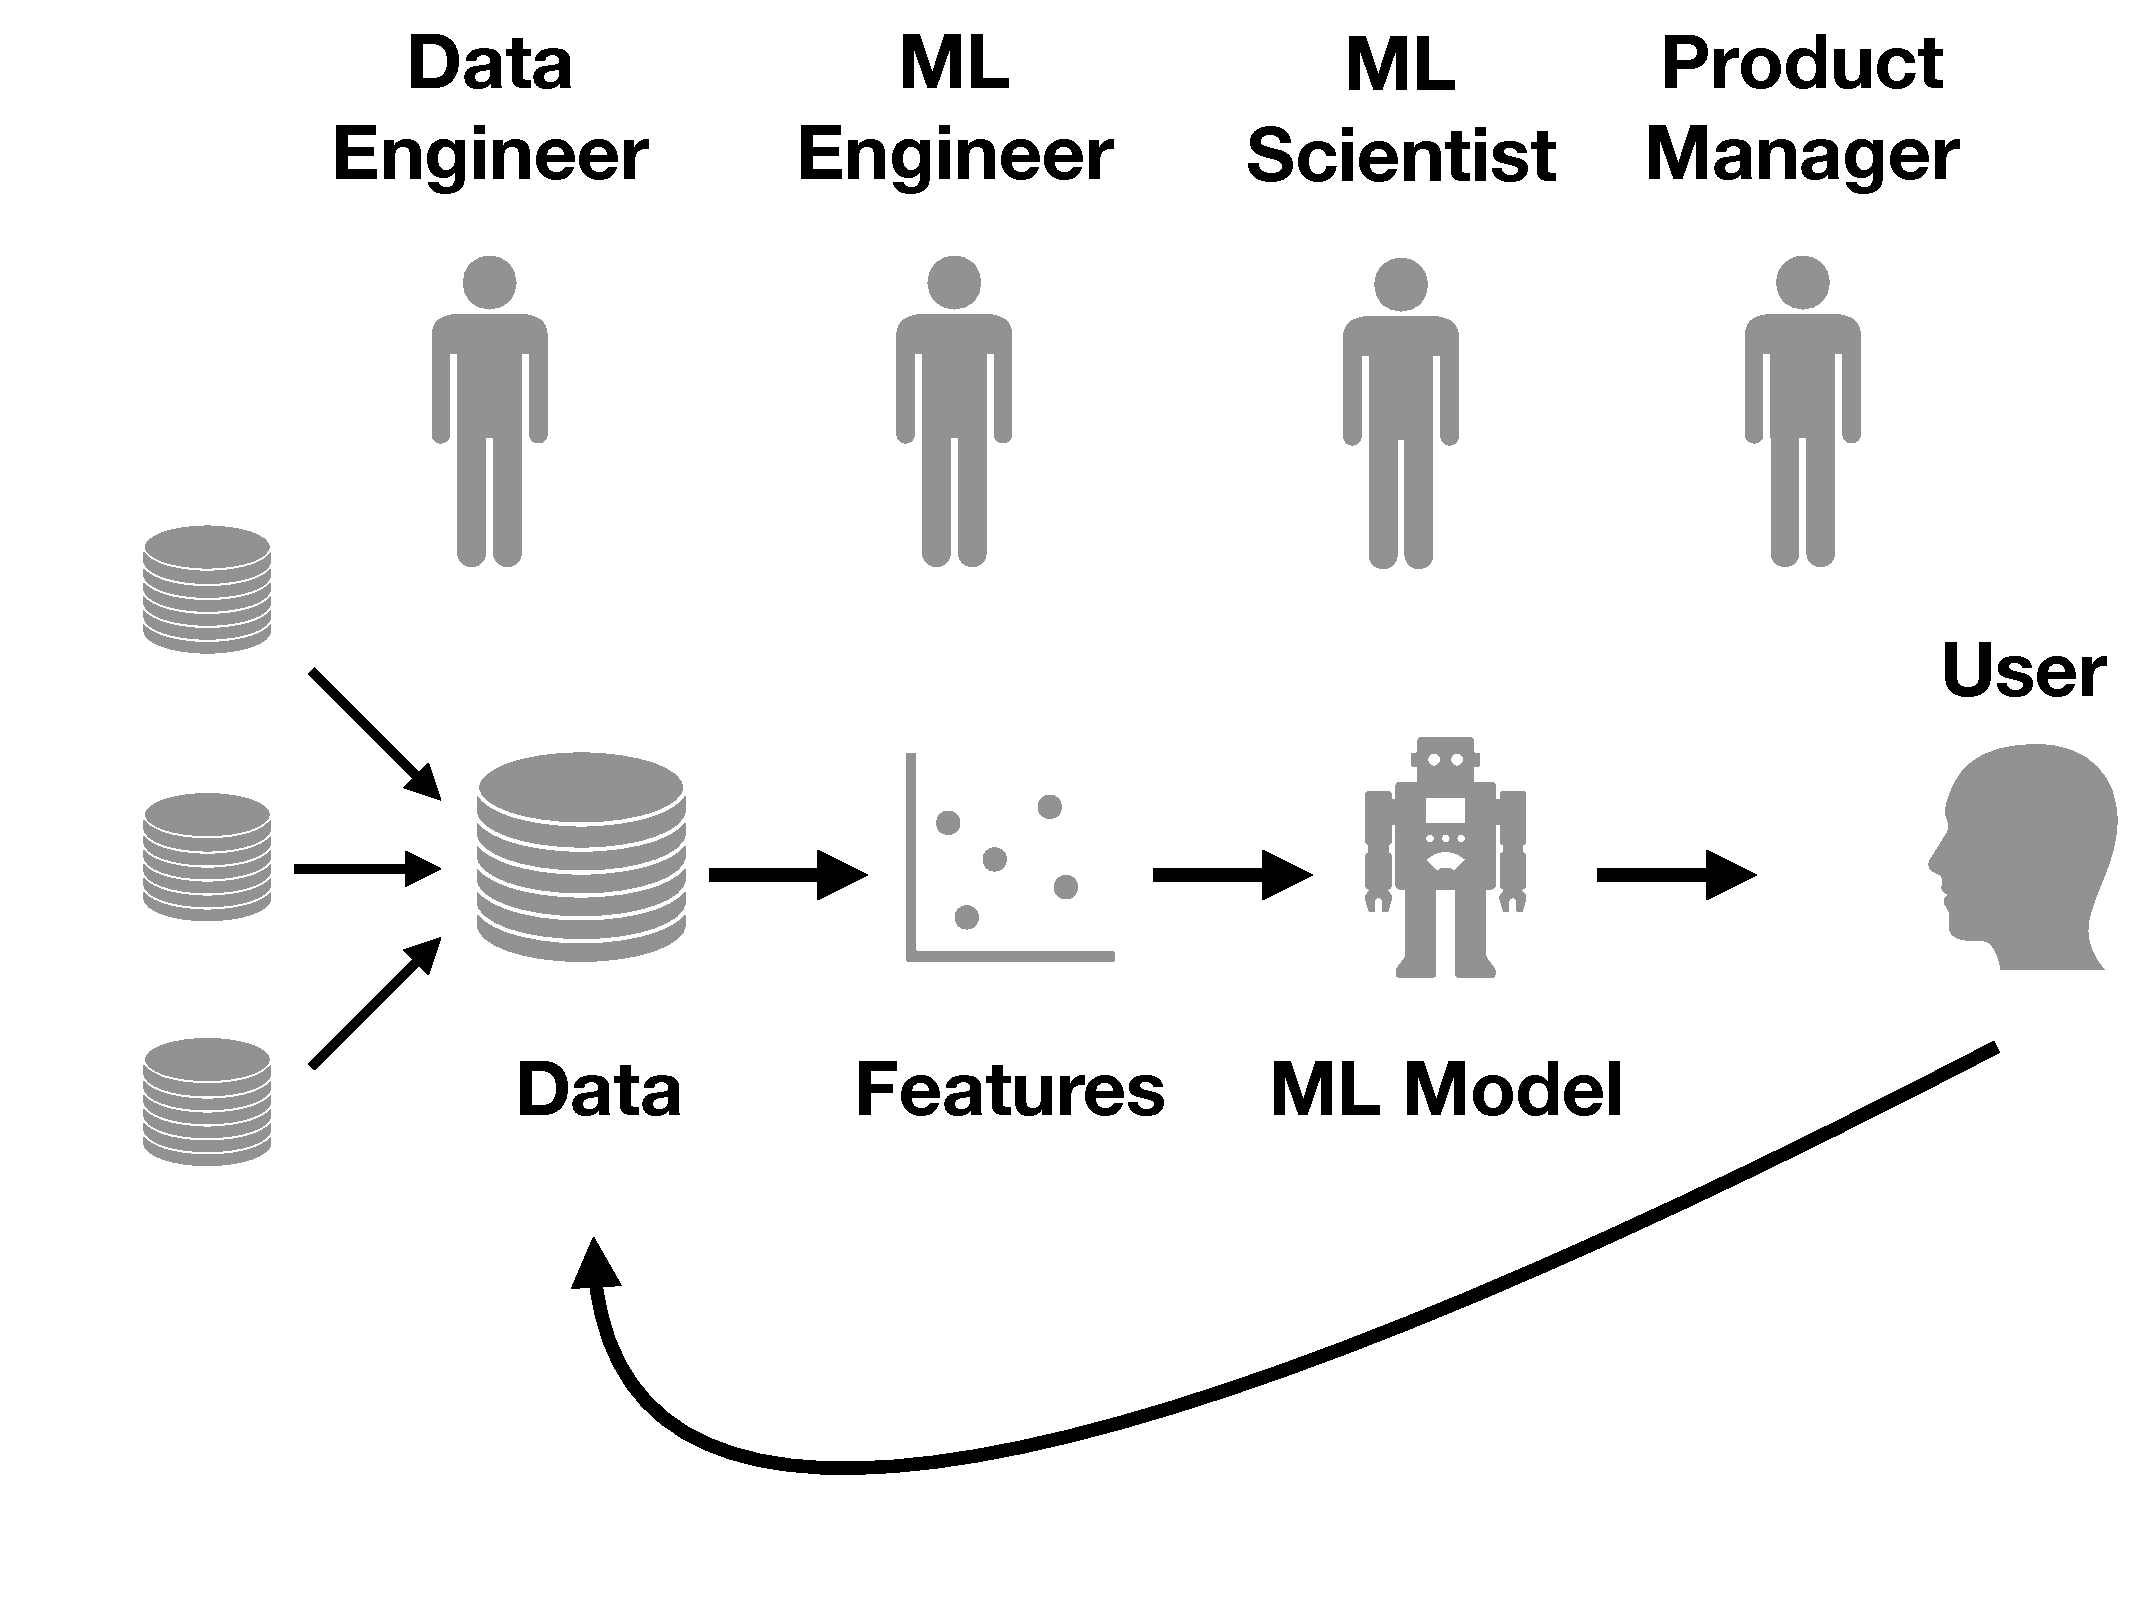
\includegraphics[width=.6\textwidth]{submissions/data-validation-amazon/figs/ML-system}
\caption{Responsibilities for a machine learning (ML) production software system are often distributed across different roles and teams \cite{Polyzotis2018}. Data from various sources is integrated, features are extracted and ML models transform these into predictions, which are then served to users whose behavioural signals are fed back to the system. Monitoring and validating these data streams at scale is only feasible with automated tests. But validating the data in each of these stages requires different competencies and often domain expertise. This imposes novel technical and conceptual challenges on engineering teams when automating ML production systems.}
\label{fig:ml-system}
\end{figure}


But why is this so difficult to automate? Researchers in the DBMS community have been investigating data profiling for decades \cite{Abedjan2018} and many of these solutions are just right for some aspects of data validation also in the context of ML systems. However some of the challenges in ML system monitoring go beyond that. Many data validation aspects in ML systems {\em depend on the state of the trained ML model}, such as the performance of a ML model under data set shift, or the differential privacy of a model \cite{Dwork08differentialprivacy, Abadi2016, Bagdasaryan2019}. Other aspects such as fairness of a ML model require domain expertise that ML engineers often do not have. As illustrated in \autoref{fig:ml-system} the competencies required to validate data in the various stages of an ML system require competencies that are usually distributed across several experts in a team or even separate teams. 

In the following chapters we will first review the challenges associated with data validation in ML systems and highlighting some of the practical implications. Afterwards we review some of the data validation solutions, with a special focus on the practical applicability of these approaches. Finally we will conclude with an outlook of technical and non-technical challenges associated with ML system validation in order to ensure more responsible usage of ML systems in production software systems. 